\documentclass{article} % For LaTeX2e
% T1 must be selected before `times'. This document is compiled with a
% XeTeX-based engine, whose default TU encoding has no descriptor for the
% ptm family: without this line every ptm shape is undefined, LaTeX
% substitutes Latin Modern silently, and \bf stops taking effect, so the
% venue's Times body text and its bold run-in headings are both lost. The
% official template was built with pdfTeX, where the question does not arise.
\usepackage[T1]{fontenc}
\usepackage{iclr2027_conference,times}

% Optional math commands from https://github.com/goodfeli/dlbook_notation.
\input{math_commands.tex}

\usepackage{hyperref}
\usepackage{url}

\usepackage{amsmath}
\usepackage{amssymb}
\usepackage{booktabs}
\usepackage{multirow}
\usepackage{graphicx}

\newcommand{\vhat}{\hat{\mathbf{v}}}
\newcommand{\yv}{\mathbf{y}}
\newcommand{\zv}{\mathbf{z}}

\title{Sanity Checks for Attention Surgery: \\
Null Models and Matched Interventions for \\
Representation-Motivated Design}

% Authors must not appear in the submitted version. The style file replaces
% this block with the anonymous notice for as long as \iclrfinalcopy stays
% commented out below.
\author{Anonymous Author \\
Anonymous Institution \\
Anonymous City, Country \\
\texttt{anon@example.invalid}
}

%\iclrfinalcopy % Uncomment for camera-ready version, but NOT for submission.
\begin{document}

\maketitle

\begin{abstract}
An attention head's output can align with its own value vector because of
both self-attention and shared representation geometry. This alignment alone
does not establish that the aligned component is redundant. We examine it
with three checks: split-half reliability of structural statistics and
intervention effects, a null using values from earlier positions, and paired
training runs with a fixed arbitrary-direction control. We measure geometry
in twelve pretrained models and intervention reliability in three. The
behavioural effect meets the reliable threshold only in GPT-2, whereas the
structural statistics are highly reliable in all three models. The
null-adjusted statistic has raw rank correlations of $0.189$ to $0.279$
with the intervention effect. In an eight-seed factorial at
$4.0\times10^{8}$ tokens per run, learned self-directed removal lowers
validation loss by $0.00292$ nats (Holm-corrected $p=0.0023$). The
arbitrary-direction arm has no statistically detectable difference from
baseline ($+0.00106$ nats, $p=0.197$). These results support a benefit from
learned self-directed removal at the tested scale, but do not establish that
the component is dispensable in a frozen model or that its cosine alignment
is a reliable guide to intervention effects.
\end{abstract}

\section{Introduction}

Multi-head self-attention \citep{vaswani2017attention} forms each head's
output as a weighted sum of value vectors. In a causal model, position $i$
can attend to its own value vector as well as to earlier positions. Exclusive
self attention (XSA) removes the output component aligned with that value
\citep{zhai2026xsa}.

\paragraph{Research objective.}
We examine whether this component is redundant and whether its cosine
alignment identifies heads whose removal changes language-modelling loss.
This is a question about a direction within a head, distinct from the
whole-head pruning studied by \citet{michel2019sixteen,voita2019analyzing}.

Two measurements are needed to interpret such an intervention. First, high
cosine alignment need not be specific to a token's own value:
contextual representations can be anisotropic \citep{ethayarajh2019contextual}.
A comparison with other values tests how much alignment survives that
background geometry. Second, an edit's loss effect must be measured
reliably before it can be related to a structural statistic. A small observed
correlation can reflect either a weak association or noisy measurements.
Training with an arbitrary-direction edit provides a further control for
whether an apparent benefit requires the own-value direction.

Our protocol addresses these questions in the following order.

\paragraph{Check 0: is the effect resolvable?} Before any correlation is
interpreted, we estimate the split-half reliability $r_\Delta$ of the
behavioural effect and $r_{\text{stat}}$ of the structural statistic. Their
geometric mean $\sqrt{r_\Delta r_{\text{stat}}}$ provides an attenuation
diagnostic. We classify the effect as reliable at $r_\Delta \ge 0.6$,
attenuated at $0.3 \le r_\Delta < 0.6$, and unresolvable below $0.3$; the
classification does not use the geometric mean as its threshold.

\paragraph{Check 1: is the self-directed cosine anisotropy?} We compare
$\cos(\yv_i, \mathbf{v}_i)$ against the same cosine computed with a null
partner drawn uniformly from earlier positions in the same sequence.
The difference measures excess alignment relative to this causal null.

\paragraph{Check 2: does the training benefit depend on direction?} We train
self-directed and arbitrary-direction arms with the same gate
parameterisation and compare each with baseline using paired seeds.
The protocol specifies the arbitrary-direction comparison as primary.

\paragraph{Contributions.}
We provide the three checks and a reconstruction gate for verifying the
captured head layout (Sections~\ref{sec:method} and \ref{sec:gate}). The
experiments comprise an eight-seed training factorial, geometry measurements
across twelve pretrained models, and reliability and correlation estimates
for three models (Sections~\ref{sec:paired} and
\ref{sec:a2}--\ref{sec:gqa}).

\section{Related Work}

\paragraph{Head importance and pruning.} \citet{michel2019sixteen} and
\citet{voita2019analyzing} show that many attention heads can be pruned with
limited degradation on their evaluated tasks. Their results concern the
importance of whole heads. We instead intervene along one direction within
each head and use an arbitrary-direction arm to test the specificity of that
choice.

\paragraph{Circuit-level accounts.} \citet{elhage2021mathematical} decompose
attention into $QK$ and $OV$ circuits and treat the diagonal of the attention
pattern as one contribution to the output. Projecting the full head output
onto its own value direction can also remove aligned contributions from
earlier tokens. It therefore differs from deleting only the diagonal term.

\paragraph{Representation geometry.} \citet{ethayarajh2019contextual} finds
anisotropy in contextual representations from ELMo, BERT, and GPT-2. This
motivates a geometric control; it does not establish the geometry of every
head examined here. Check~1 measures that background using values from
earlier positions in the same sequence.

\paragraph{Isotropy is not universal.} \citet{timkey2021bark} show that a
small number of high-variance coordinates dominate cosine similarity in
contextual spaces, so a raw cosine can be large without reflecting shared
structure. \citet{machina2024anisotropy} further report that the large Pythia
models have approximately isotropic embedding spaces, which bounds how much a
generic anisotropy argument can explain. Our null is computed within the same
run, at one stated sequence length, on the same documents as the observed
statistic, so it measures the earlier-position background of each model
directly rather than assuming a uniform anisotropy across the ladder.
%% AUTHOR CHECK: your README argues the ladder answers this directly (a large
%% share of cos(y_i, v_i) remains attributable to the null even at 6.9B).
%% That quantified rebuttal is currently absent from the paper. Verify the
%% figure against results/ and add it here if it holds.

\paragraph{Grouped-query attention.} \citet{ainslie2023gqa} share key and value
projections across groups of query heads. We compare own-group and
neighbouring-group values to assess the statistic's dependence on that sharing in
Section~\ref{sec:gqa}.

\section{Method}
\label{sec:method}

\subsection{The intervention}

Let head $h$ at layer $\ell$ produce output $\yv_i \in \mathbb{R}^{d_h}$ at
position $i$, and let $\mathbf{v}_i$ be the value vector that same head writes
at $i$. Write $\vhat_i = \mathbf{v}_i / \lVert \mathbf{v}_i \rVert$. The
self-directed removal, which we call XSA, replaces the head output with
%
\begin{equation}
\zv_i \;=\; \yv_i \;-\; \tanh(\alpha)\,\langle \yv_i, \vhat_i\rangle\,\vhat_i ,
\label{eq:xsa}
\end{equation}
%
where $\alpha$ is a gate for each layer and head. The edit acts before the
output projection. For frozen models, we set the multiplier to one and
intervene on one head at a time, excluding the first token. In the trained
factorial, gates start at zero and are learned jointly with the model; all
positions are included. A zero gate disables the edit, and a negative gate
adds an aligned component. The implementation stabilises normalisation by
using $\mathbf{v}_i/(\lVert\mathbf{v}_i\rVert+\epsilon)$, with
$\epsilon=10^{-8}$ for frozen measurements and $10^{-6}$ for training.
Equation~\ref{eq:xsa} states the idealised unit-direction form.

The \textsc{random} control uses the same gated edit with a fixed arbitrary
direction for each layer and head. Directions are sampled by normalising
isotropic Gaussian vectors, seeded by layer index, and held fixed across
positions, training steps, and run seeds. Both arms use the same normalisation
and gate parameterisation, but their projection magnitudes need not match.
The harness also implements \textsc{meanval} and \textsc{diagmask}
(Appendix~\ref{app:arms}); neither appears in the reported three-arm factorial.

\subsection{Check 0: resolvability}

Split the evaluation corpus into halves $A$ and $B$ and measure each head's
effect $\Delta$ and structural statistic on both halves. Spearman
correlations across heads give the split-half reliabilities $r_\Delta$ and
$r_{\text{stat}}$. The archived analysis applies no Spearman--Brown
correction and reports:
%
\begin{equation}
\rho_{\max} \;=\; \sqrt{r_\Delta \, r_{\text{stat}}},
\qquad
\rho_{\text{disatt}} \;=\; \rho_{\text{raw}} / \rho_{\max}.
\label{eq:ceiling}
\end{equation}
%
We classify the effect as reliable at $r_\Delta \ge 0.6$, attenuated at
$0.3 \le r_\Delta < 0.6$, and unresolvable below $0.3$. An unresolvable
effect does not support interpreting a small correlation as absence of an
association. Each structural statistic uses its own reliability estimate.

For $\rho_{\text{raw}}$, the statistic and effect are each averaged across
the two halves before computing their Spearman correlation across heads.
Because the denominator in Equation~\ref{eq:ceiling} uses half-sample
reliabilities, the adjusted value is a diagnostic, not a calibrated estimate
of the latent correlation between the pooled measurements. We retain the
archived notation $\rho_{\max}$, but do not interpret it as a strict bound
on those pooled correlations.

\subsection{Check 1: the anisotropy null}

For each head and position, $\cos(\yv_i, \mathbf{v}_i)$ is compared against
$\cos(\yv_i, \mathbf{v}_j)$ with $j$ drawn uniformly from
$\{1,\dots,i-1\}$ using one-based indexing. The first token is excluded
because it has no earlier partner and its head output equals its own value.
The statistic, \emph{excess}, is the mean paired difference between the
cosines. It controls for alignment with earlier values, not all sources of
anisotropy. The model-ladder figure reports point estimates; the harness
supports layer-cluster bootstrap intervals for head-level data.

\begin{samepage}
Two further diagnostics use different nulls. For attention sinks, we compare
attention mass on the first token with the average mass on the next three
tokens, using queries from the ninth token onward. For massive activations,
we compare the mean maximum absolute hidden coordinate, scaled by the hidden
tensor's standard deviation, with the Gaussian reference
$\sqrt{2\log d}$ for width $d$. This reference is a scale approximation,
not an exact finite-width expected maximum.
\end{samepage}

\subsection{Check 2: matched intervention}
\label{sec:check2}

Check~2 is run as a paired factorial over seeds. For each seed, all arms train
from an identical initialisation on an identical token stream, so the paired
difference controls for variation shared within a seed. Define $\Delta$ as
the arm's validation loss minus baseline loss, so negative values indicate
improvement. The protocol-specified primary endpoint is \textsc{random}
versus baseline. The XSA comparison is secondary, with Holm correction
\citep{holm1979simple} restricted to secondary endpoints. XSA is the only
secondary in the completed factorial, so its adjusted and unadjusted
$p$-values coincide. We report two-sided paired $t$-tests and percentile
bootstrap intervals over seed differences. Separate baseline comparisons
do not constitute a direct test of XSA against \textsc{random}.

The analysis approximates the minimum detectable effect at $80\%$ power and
$\alpha = 0.05$ by
%
\begin{equation}
\text{MDE} \;=\; 2.9\,\sigma_{\text{paired}} \big/ \sqrt{n},
\label{eq:mde}
\end{equation}
%
using the observed $\sigma_{\text{paired}}$. We call this the realised MDE
to distinguish it from the planning forecast. It describes sensitivity under
the approximation, not achieved power or a hard threshold for detection.

\subsection{The reconstruction gate}
\label{sec:gate}

A head-layout error can preserve tensor shape while changing the intervention.
We rebuild $\yv = A\,\mathrm{expand\_kv}(V)$ from the captured attention
matrix and values, then compare it with the input to the output projection.
The gate rejects a relative Frobenius error above $10^{-2}$ or a non-finite
value. In each reliability run, it checks the first, middle, and last layers
on one document before measuring head effects.

The implementation notes record an initial Pythia-160M error of
$2.0\times10^{-4}$ and errors of $1.39$ to $1.50$ after reversing heads,
rolling the head axis, or omitting a transpose. These observations motivated
the threshold. In the archived reliability runs, the maximum error across
the checked layers is approximately $1.6\times10^{-3}$ for each model,
below the same threshold. A passed gate supports the tensor reconstruction
at those checked layers; it does not validate the intervention's semantic
interpretation.

\section{Experimental Setup}

\paragraph{Frozen-model measurements.} Check~1 covers twelve pretrained
models, including nine multi-head models from $124$M to $6.9$B parameters
and three grouped-query models. These include the GPT-2
family \citep{radford2019language} and the Pythia suite
\citep{biderman2023pythia}. Model revisions are recorded by hash. The
geometry measurements use WikiText-103 test documents and each run's recorded
block length. Check~0 is restricted to GPT-2, Pythia-160M, and Pythia-410M,
using $64$ documents per half at a fixed length of $128$ tokens. Shorter
documents are dropped rather than padded. This length constraint applies to
the reliability runs, not to the full model ladder.

\paragraph{Trained factorial.} Check~2 uses a decoder-only model with eight
layers, eight heads per layer, and hidden width $512$, approximately $50.9$M
parameters. The data pipeline uses FineWeb-Edu's sample-10BT stream with a
fixed disjoint validation holdout. We trained from scratch on eight seeds
(7, 42, 99, 512, 1337, 2024, 8191, 31337) under three
arms (\textsc{baseline}, \textsc{xsa}, \textsc{random}), giving 24 cells.
Each cell sees $399\,900\,672$ tokens, rounded down from the budget to a
whole number of batches. Runs share initialisation, token order, learning-rate
schedule, and validation batches within each seed. All three arms for a seed
complete before the next seed starts.

\paragraph{Budget.} The completed factorial cost \$15.58 against a \$20
ceiling. The ledger records $16.98$ GPU-hours spent in training cells;
billing covers pod uptime, including time outside those cells. An earlier
$5\times10^{7}$-token pilot is retained separately and is not pooled with
the primary runs.

\section{Results}

\begin{table}[tb]
\centering
\small
\begin{tabular}{@{}lrrrl@{}}
\toprule
Model & $r_\Delta$ & $r_{\text{stat}}$ & $\rho_{\max}$ & Verdict \\
\midrule
GPT-2         & 0.795 & 0.997 & 0.890 & reliable \\
Pythia-160M   & 0.419 & 0.994 & 0.645 & attenuated \\
Pythia-410M   & 0.531 & 0.991 & 0.726 & attenuated \\
\bottomrule
\end{tabular}
\caption{Check~0 split-half reliability, $n = 144$ heads for GPT-2 and
Pythia-160M and $n = 384$ for Pythia-410M, at a fixed sequence length of $128$
tokens with $64$ documents per half. The verdict uses $r_\Delta$;
$r_{\text{stat}}$ here refers to self-cosine. $\rho_{\max}$ is the
attenuation factor in Equation~\ref{eq:ceiling}.}
\label{tab:reliability}
\end{table}

\begin{table}[tb]
\centering
\small
\begin{tabular}{@{}llrrr@{}}
\toprule
Model & Statistic & $\rho_{\text{raw}}$ & $\rho_{\max}$ & $\rho_{\text{disatt}}$ \\
\midrule
\multirow{2}{*}{GPT-2}
  & self-cosine & $+0.462$ & 0.890 & $+0.519$ \\
  & excess      & $+0.279$ & 0.891 & $+0.313$ \\
\multirow{2}{*}{Pythia-160M}
  & self-cosine & $+0.149$ & 0.645 & $+0.231$ \\
  & excess      & $+0.189$ & 0.646 & $+0.292$ \\
\multirow{2}{*}{Pythia-410M}
  & self-cosine & $-0.025$ & 0.726 & $-0.034$ \\
  & excess      & $+0.249$ & 0.727 & $+0.342$ \\
\bottomrule
\end{tabular}
\caption{Spearman correlation between the structural statistic and the measured
behavioural effect, raw and adjusted using Equation~\ref{eq:ceiling}.
The raw correlation uses averages over both halves; the adjustment uses
each statistic's own half-sample reliability.}
\label{tab:a2}
\end{table}

\begin{table}[tb]
\centering
\small
\begin{tabular}{@{}lrr@{}}
\toprule
 & \textsc{random} & \textsc{xsa} \\
 & (primary) & (secondary) \\
\midrule
Mean $\Delta$ (nats)     & $+0.001056$ & $-0.002924$ \\
CI low                   & $-0.000298$ & $-0.003967$ \\
CI high                  & $+0.002390$ & $-0.001709$ \\
$t$                      & $+1.43$     & $-4.67$ \\
$p$                      & $0.197$     & $0.0023$ \\
Holm $p$                 & n/a         & $0.0023$ \\
Cohen's $d_z$            & $+0.504$    & $-1.649$ \\
$\sigma_{\text{paired}}$ & $0.002095$  & $0.001773$ \\
Realised MDE             & $0.00215$   & $0.00182$ \\
\bottomrule
\end{tabular}
\caption{Check~2, eight complete paired seeds, $399\,900\,672$ tokens per run.
Both contrasts are against \textsc{baseline}. Positive $\Delta$ means higher
loss. Intervals are $95\%$ percentile bootstrap intervals over paired seed
differences. The realised MDE uses the observed $\sigma_{\text{paired}}$.
Holm correction does not apply to the primary endpoint.}
\label{tab:paired}
\end{table}


% Every figure is declared here rather than beside the paragraph that
% discusses it. A float can only land on or after the page it is declared on,
% and with ten of them the deferral compounds: declared in place, figures were
% surfacing two pages after their first mention. reflow_floats.py did the move
% and check_floats.py measures the result.
\begin{figure}[tb]
\centering
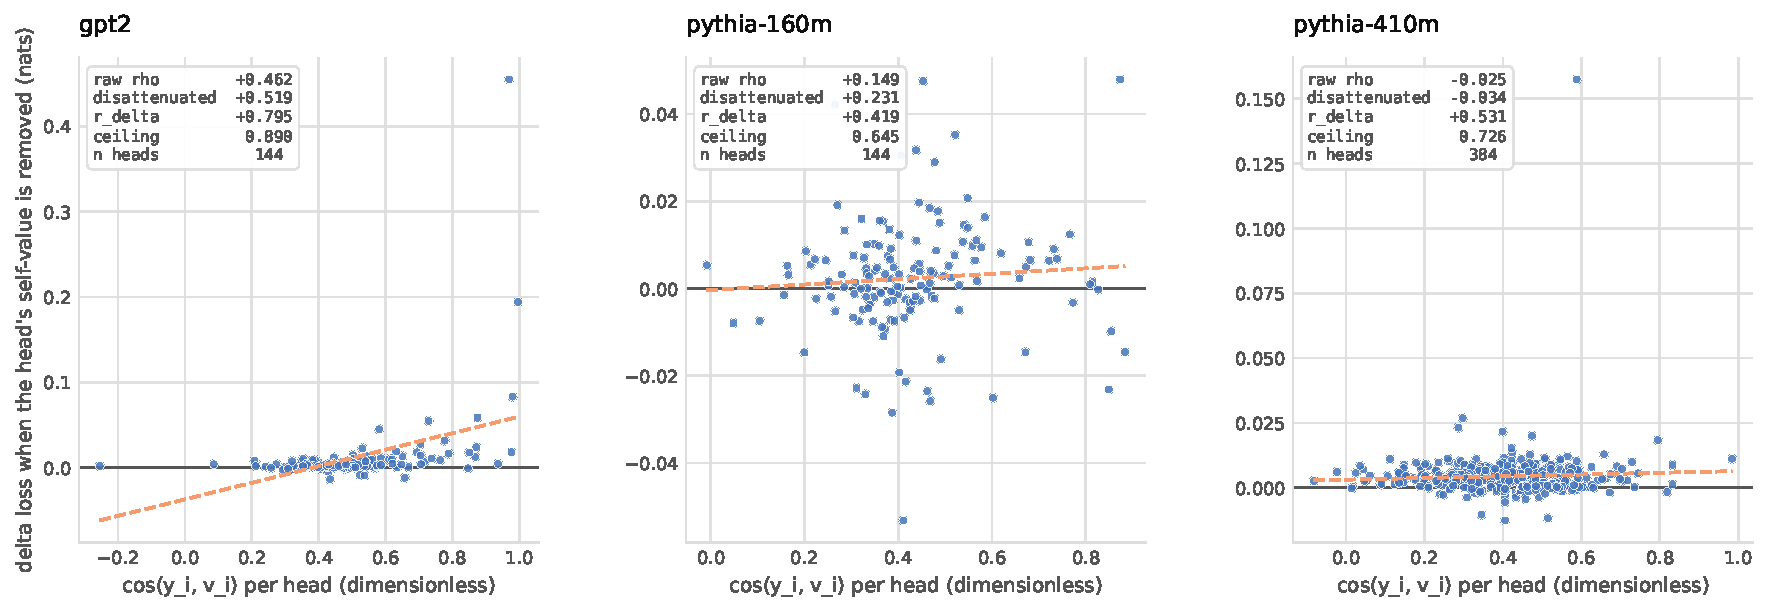
\includegraphics[width=0.98\linewidth]{figs/fig6_a2_scatter.pdf}
\caption{Self-cosine against the loss effect of frozen-head intervention.
Points use the half-A statistic and the effect averaged over both halves;
panel annotations report the pooled-statistic correlations in
Table~\ref{tab:a2}. Dashed least-squares lines are visual guides, not tests
of significance. Vertical scales differ across panels.}
\label{fig:a2}
\end{figure}

\begin{figure}[tb]
\centering
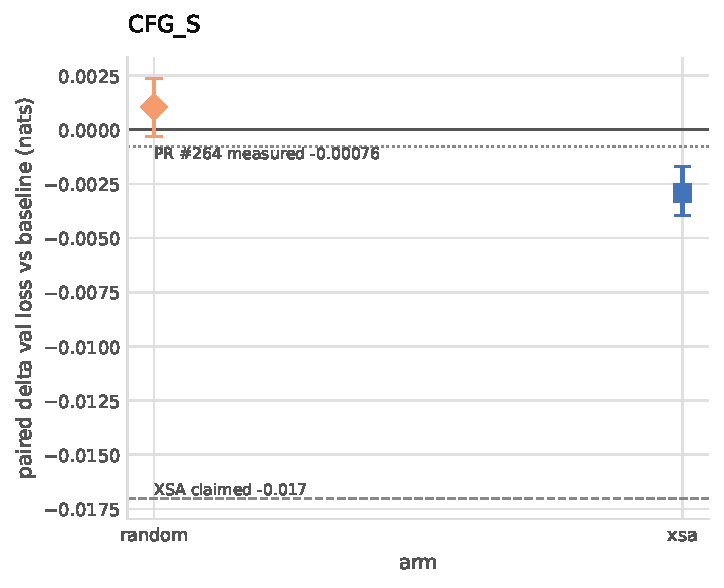
\includegraphics[width=0.42\linewidth]{figs/fig2_paired_delta.pdf}
\caption{Paired difference in validation loss against baseline, with $95\%$
intervals, over eight paired seeds. The \textsc{random} interval crosses zero
and the \textsc{xsa} interval lies below zero. The horizontal reference
lines retain the project's external reference values. The $-0.00076$ value
comes from the H200 comparison in
\href{https://github.com/KellerJordan/modded-nanogpt/pull/264}{PR~\#264},
which uses different training step counts between arms. The exact source
configuration for $-0.017$ is unresolved. Neither is a matched replication
target for this experiment.}
\label{fig:paired}
\end{figure}

\begin{figure}[tb]
\centering
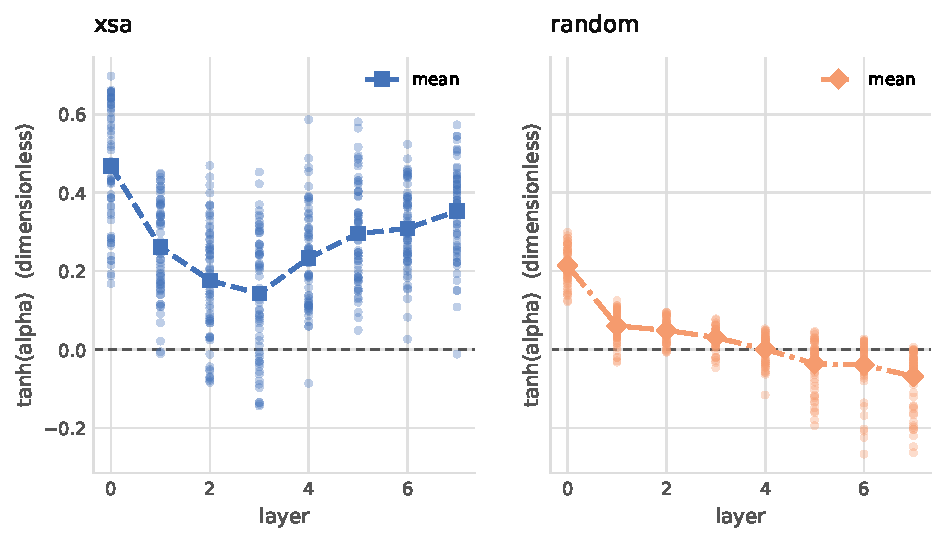
\includegraphics[width=0.55\linewidth]{figs/fig1_gates.pdf}
\caption{Final learned gates $\tanh(\alpha)$ for all heads and seeds, with
markers at the layer mean. XSA has positive means at every layer. The
\textsc{random} mean approaches zero by layer four and becomes negative
in later layers. A negative gate adds the projected component. These are
endpoint measurements, not gate trajectories during training.}
\label{fig:gates}
\end{figure}

\begin{figure}[tb]
\centering
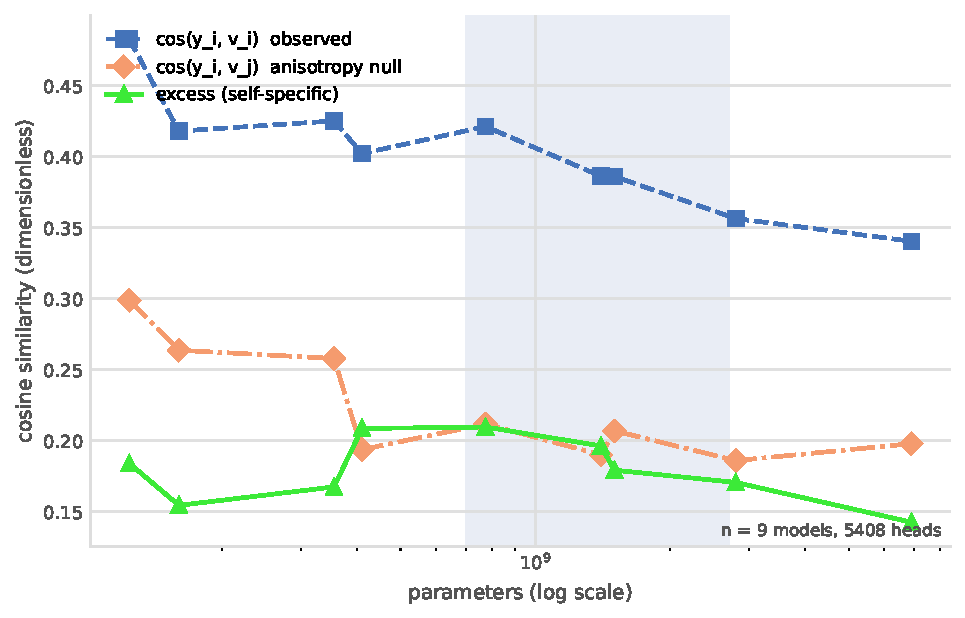
\includegraphics[width=0.50\linewidth]{figs/fig3_ladder.pdf}
\caption{Check~1 across the nine multi-head models in the ladder, every model
pinned by revision hash. Observed $\cos(\yv_i,\mathbf{v}_i)$, the anisotropy
null $\cos(\yv_i,\mathbf{v}_j)$, and their difference. The observed curve
generally declines with scale; the excess has no monotone trend.}
\label{fig:ladder}
\end{figure}

\begin{figure}[tb]
\centering
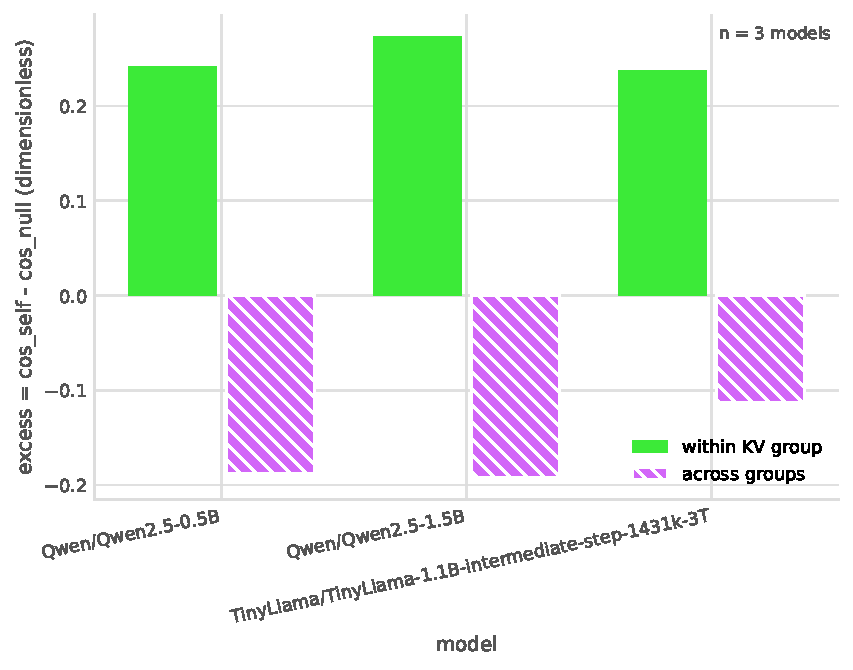
\includegraphics[width=0.48\linewidth]{figs/fig5_gqa.pdf}
\caption{Within-group against across-group excess for the three grouped-query
models. Both subtract the own-group earlier-position null. Own-group excess
is positive and neighbouring-group excess negative in all three models.
The harness does not report this grouping contrast for multi-head models.}
\label{fig:gqa}
\end{figure}


\subsection{Resolvability}

The behavioural effect is reliable in GPT-2 and attenuated in both Pythia
models under the Check~0 thresholds (Table~\ref{tab:reliability}). None of
the three is classified as unresolvable. Structural self-cosine reliability
is high in all three, from $0.991$ to $0.997$. The main source of attenuation
is therefore the intervention-effect measurement. For Pythia-160M, dividing
the raw self-cosine correlation of $0.149$ by the diagnostic factor $0.645$
gives $0.231$; this adjustment does not remove the uncertainty associated
with an attenuated effect.

\subsection{Structural statistic versus behavioural effect}
\label{sec:a2}

The relation between self-cosine and the measured effect varies by model
(Figure~\ref{fig:a2}, Table~\ref{tab:a2}). GPT-2 has a raw correlation of
$+0.462$ and an adjusted value of $+0.519$; Pythia-410M has an adjusted
value of $-0.034$, close to zero. For excess, the adjusted correlations are
$+0.313$, $+0.292$, and $+0.342$ across the three models. These are
descriptive rank associations, not estimates of explained loss variance or
out-of-sample predictive accuracy.

An earlier Pythia-160M run reported a raw excess correlation of $+0.487$,
compared with $+0.189$ in the current run. Several protocol changes
accompanied the rerun (Appendix~\ref{app:deviations}), so their individual
contributions to this difference are not isolated.

\subsection{The paired factorial}
\label{sec:paired}

All 24 training cells completed, giving eight paired seeds for each contrast
in Table~\ref{tab:paired} and Figure~\ref{fig:paired}.

For the primary endpoint, the \textsc{random} arm's loss difference is
$+0.001056$ nats ($p = 0.197$). Its $95\%$ interval,
$[-0.000298, +0.002390]$, includes both a small benefit and a small loss
increase. The result is nonsignificant, without establishing equivalence.

The secondary endpoint, \textsc{xsa} versus baseline, is $-0.002924$ nats with
interval $[-0.003967, -0.001709]$, $t = -4.67$, and Holm-corrected $p =
0.0023$. XSA therefore lowers loss in this training setting. The realised MDE from
Equation~\ref{eq:mde} is $0.00182$ nats for the XSA contrast and $0.00215$ for
the control contrast. The observed XSA effect is about $1.6\times$ its
approximate MDE, whereas the control effect is smaller than its MDE.
Figure~\ref{fig:power} shows sensitivity estimates for the control at both
token budgets.

The benefit concerns a model trained with learned removal. It does not show
that the same component can be removed from an already trained model without
cost, or establish a direct between-arm difference from the separate tests.

Final gates differ between arms (Figure~\ref{fig:gates}). XSA's layer means
range from $0.14$ to $0.47$, indicating partial removal on average.
The control's later-layer means are negative, indicating addition along
its direction. These endpoint measurements do not explain the loss difference.

\subsection{Check 1 across the model ladder}
\label{sec:ladder}

Across nine multi-head models and $5408$ heads, self-cosine generally
declines with model size (Figure~\ref{fig:ladder}). It is $0.483$ for
GPT-2 at $124$M parameters and $0.340$ for Pythia-6.9B. The earlier-position
null also declines overall. Excess remains between $0.14$ and $0.21$
without a monotone trend. These observations do not establish scale
invariance, but show that the raw cosine's trend is partly shared by its
null. The grouped-query models are examined separately below.

Both additional GPT-2 diagnostics exceed their respective nulls
(Figure~\ref{fig:generality}). Attention mass on the first token is
$0.403$, compared with $0.003$ on the matched early positions. The
massive-activation statistic is $12.87$ against a Gaussian reference of
$3.65$, leaving approximately $71.7\%$ after subtraction. Neither pattern
is explained away by its chosen null. The two unexecuted diagnostics are
shown as blank categories.

\subsection{Grouped-query attention}
\label{sec:gqa}

For each grouped-query model, we compare the head output's cosine with its
own group's value and with a neighbouring group's value at the same position.
Both excess values subtract the own-group earlier-position null. For
Qwen2.5-0.5B ($14$ query heads over $2$ key--value heads), own-group excess
is $+0.2415$ and neighbouring-group excess is $-0.1876$. Qwen2.5-1.5B
and TinyLlama-1.1B show the same signs (Figure~\ref{fig:gqa}). The
alignment thus depends on which group's value is used. A negative
across-group excess means alignment below the own-group null, not
necessarily a negative raw cosine. The harness leaves this contrast
undefined for multi-head models, which lack groups sharing a value
projection.

\section{Limitations}

\paragraph{Training and scale.} Check~2 measures adaptation in a small model
trained for $4.0\times10^{8}$ tokens per run. It does not establish the
effect's sign or magnitude at larger scales. The frozen and trained
experiments also differ in gate strength and first-token treatment, so their
effects are not estimates of the same intervention.

\paragraph{One statistic family.} Both structural statistics are cosine-based.
A statistic based on attention mass could have a different relation to
intervention effects. The present analysis does not test that alternative.

\paragraph{Reliability and correlation.} Only three models underwent
Check~0. Reliability for the other nine remains unmeasured, and the
disattenuation uses half-sample reliabilities for pooled correlations.
The adjusted values should therefore be read alongside the raw values,
not as corrected ground truth. Neither rank correlations nor the fitted
scatterplot lines establish predictive accuracy.

\paragraph{Control scope.} The random and XSA arms share a rank-one form,
but their removed norms and final gates differ. The trained comparison does
not isolate norm from direction. Reconstruction checks validate selected
tensor layouts, not the claim that a value-aligned projection contains only
self-position information.

\paragraph{Reference mismatch.} The GPT-2 geometry measurement did not
reproduce the project's reference triple within its stated tolerance of
$0.01$. At block $512$ the measured self-cosine, null, and excess were
$0.4828$, $0.2987$, and $0.1840$, against reference values $0.5406$,
$0.3798$, and $0.1608$.

A length sweep accounts for most of that gap. The reference triple is quoted
without a sequence length, and the null is strongly length-dependent while the
observed self-cosine is close to flat. Across $64$ to $1024$ tokens the null
moves by $0.096$, nine times the tolerance, and at $64$ tokens it sits $0.005$
from the reference value, inside it. The excess moves by $0.080$ and comes
within $0.011$ at $256$ tokens. The self-cosine moves by only $0.016$ and
never comes within $0.051$, so length does not account for that component; its
residual gap is consistent with a difference in corpus, truncation, or
head-level aggregation, and we have not identified which.

The consequence for Check~1 is narrow. The null is measured inside the same
runs, at one stated length, on the same documents as the observed statistic,
so the comparison the check makes is internally matched whatever the absolute
level. The excess is positive at every length tested. What the sweep does show
is that a self-specific fraction quoted without a length is not comparable
across studies: the same GPT-2 gives $0.235$ at $64$ tokens and $0.412$ at
$1024$. We therefore report the length everywhere and do not claim
reproduction of the reference triple.

\section{Conclusion}

Learned self-directed removal improves validation loss by $0.0029$ nats in
the eight-seed factorial, with Holm-corrected $p = 0.0023$. The fixed
arbitrary-direction arm has no statistically detectable difference from
baseline. This supports the trained XSA variant at the tested scale, while
leaving open whether its benefit generalises or reflects redundancy in a
frozen model.

Own-value alignment exceeds an earlier-position null, but its association
with intervention effects varies across models. Excess has modest rank
correlations in all three examined. Interpreting such associations requires
reliable effect measurements as well as a control suited to the intervention.

\subsection*{AI use statement}

AI assistants were used during the development of this work. The authors
defined the research question, experimental design, methodological choices, and
interpretation of results. AI-assisted code was reviewed and validated by the
authors, and reported results were verified against the stored result files.
The authors take responsibility for every claim, citation, and number in this
paper. Use by category:

\begin{itemize}
\setlength{\itemsep}{2pt}
\item \textbf{Synthetic data.} None. All text is public corpora; no generated
data enters any result.
\item \textbf{Hypotheses.} Author-defined. The research question, the
three checks, and the pre-registered primary endpoint were specified by the
authors before any assistant was involved in the experimental programme.
%% AUTHOR CHECK: confirm this is accurate before submitting.
\item \textbf{Theory, proofs, and conceptual frameworks.} None. The paper
contains no theorem or proof, and the conceptual framing of the three checks
is author-originated.
\item \textbf{Methodology and experiment design.} Author-defined. Assistants
enumerated candidate controls and failure modes and drafted the power and
token-budget arithmetic, which the authors reviewed before adoption.
\item \textbf{Core code.} Assistant-written under author direction: the
intervention, null sampling, the reconstruction gate, the statistical
routines, the experiment drivers, and the tests. The authors reviewed it and
specified the guards. Defects found this way are recorded in the repository.
\item \textbf{Data cleaning and analysis.} Assistant-implemented from
author-specified definitions. Every table cell and manifest claim is
recomputed from the stored files by a checker rather than transcribed.
\item \textbf{Interpreting results.} Author-owned. Assistants were used
adversarially against the draft, and a second model from a different vendor
reviewed the analysis; both surfaced errors the authors then corrected,
including a reversed sign convention in an earlier draft.
\item \textbf{Figures.} All figure code is assistant-written and reads only
from the stored result files. No figure content was drawn or edited by hand.
\item \textbf{Writing and editing.} The manuscript was drafted with assistant
help and revised by the authors, who also used assistants to check the draft
against the archived results and the cited sources.
\item \textbf{Translation.} None. The work was written in English throughout.
\item \textbf{Literature search, references, and structure.} Assistants were
used for literature search and summarisation, reference formatting, and
suggestions on section structure and title wording. The authors verified every
cited work against its original source.
%% AUTHOR CHECK: these are recommended-disclosure tasks. Amend to match what
%% actually happened; delete any that did not.
\end{itemize}

\subsection*{Ethics statement}

This work analyses the internal structure of publicly released pretrained
language models and trains small models from scratch on public text. It
introduces no new data collection, no human subjects, and no deployed system.
The small-model training result does not establish that attention components
can be pruned safely in deployed models. Any such use requires evaluation in
the intended model and setting.

\subsection*{Reproducibility statement}

The repository contains per-run factorial records, paired-test summaries,
per-head geometry and intervention measurements, and revision hashes for all
twelve pretrained models. Code for the intervention, null sampling,
reconstruction gate, and statistical calculations accompanies the results.
The pilot runs are stored apart from the primary factorial and are labelled
as such. An anonymised copy of the repository is available at
\url{ANONYMOUS-ARTIFACT-URL}.
%% AUTHOR ACTION: replace with an anonymous.4open.science mirror, or upload the
%% code as supplementary material. Do NOT paste the GitHub URL: it contains
%% your username and breaks double-blind review.

Every figure is generated from these stored results. The tables are written by
hand, so a checker recomputes each of their 48 cells from the archived result
files and compares against the printed value at the precision shown. Cells
that the manuscript derives are recomputed rather than read back:
$\rho_{\max}$ from its two reliabilities, $\rho_{\text{disatt}}$ from the raw
correlation and that factor, and the realised MDE from the observed paired
standard deviation and seed count. Tables 1--3 currently agree with their
sources on all 48 cells. The checker also reports any table row it does not
know how to verify, so an unchecked row cannot pass silently.

Separately, a manifest recomputes 31 numerical claims from the committed
artifacts and fails on any that does not reproduce within a stated tolerance.
All 31 reproduce at the commit this manuscript was built from.

\bibliographystyle{iclr2027_conference}
\bibliography{references}

\appendix

% Moved here to keep the main text within the nine-page limit.
% Both figures' numbers are stated in the sections that cite
% them, so nothing is lost from the argument by their position.
% See move_to_appendix.py.
\begin{figure}[tb]
\centering
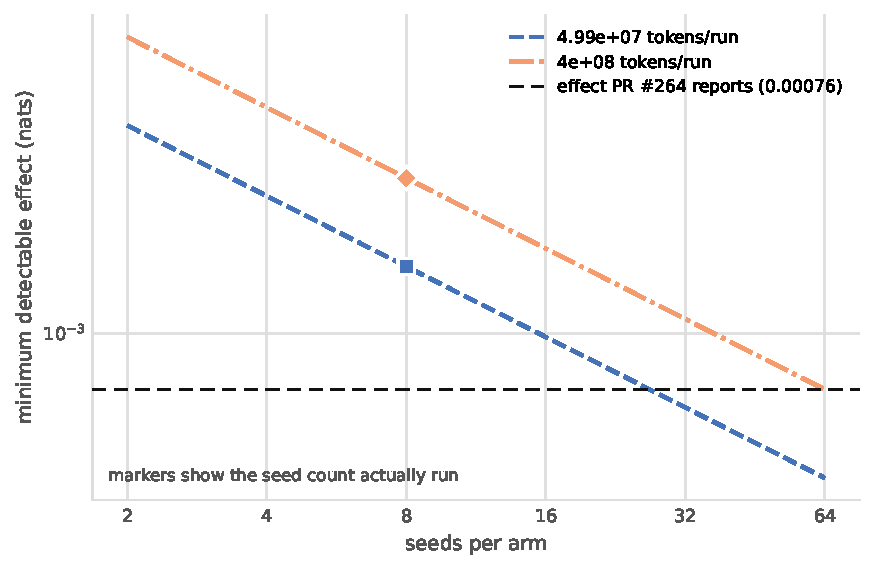
\includegraphics[width=0.50\linewidth]{figs/fig7_power.pdf}
\caption{Approximate MDE for the \textsc{random}-versus-baseline contrast,
using the observed paired standard deviation at each token budget. Markers
show the eight seeds actually run; the remaining points extrapolate at fixed
variance. Both eight-seed estimates exceed the external reference magnitude
of $0.00076$ nats from the PR~\#264 comparison described in
Figure~\ref{fig:paired}.}
\label{fig:power}
\end{figure}

\begin{figure}[tb]
\centering
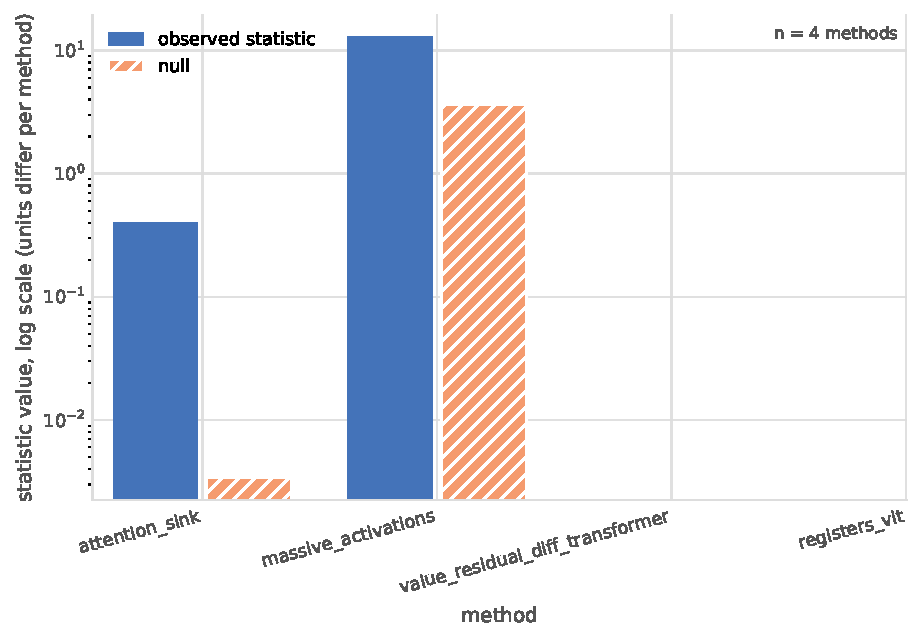
\includegraphics[width=0.48\linewidth]{figs/fig4_generality.pdf}
\caption{Observed statistics and their respective nulls for two GPT-2
diagnostics: attention mass for attention sinks and standard-deviation units
for massive activations. Both exceed their nulls. The logarithmic axis
accommodates different magnitudes; values across diagnostics have different
units. The two blank categories were not run: one requires training matched
models, and the other requires a vision-model harness.}
\label{fig:generality}
\end{figure}


\section{Arm Definitions}
\label{app:arms}

\textsc{baseline} leaves the head output unchanged. \textsc{xsa} uses
Equation~\ref{eq:xsa}, with a learned gate in the factorial and a unit
multiplier in the frozen-head measurements. \textsc{random} substitutes a
fixed arbitrary direction per layer and head and learns the same type of gate.

The two additional harness arms were not evaluated in the primary factorial.
\textsc{meanval} uses a detached exponential moving average of the head's
batch-mean value, updated only during training. \textsc{diagmask} operates
on logits. Its default gated form subtracts $30\tanh(\alpha)$ from diagonal
logits before softmax; the optional hard-mask form sets them to $-\infty$.
Both leave the first token unmasked because it has no alternative key.
These implementations should not be read as completed experimental arms.

\section{Budget Ledger}
\label{app:budget}

The ledger records completed seed blocks and separates training-cell time
from billed pod uptime. Adding cell hours to uptime would count training
twice. An earlier forecast of \$18.16 made that error; the corrected
projection at the same stage was \$13.41. The final billed total was
\$15.58.

\section{Changes to the Measurement Protocol}
\label{app:deviations}

The reliability runs now use a fixed length of $128$ tokens. Earlier runs
allowed the common length to depend on the selected documents: $142$ tokens
at $24$ documents per half and $137$ at $64$. This changes the null partner
set as well as the measurement budget. The analysis also now pools both
halves of the statistic and effect and uses statistic-specific reliability
for disattenuation. The earlier Pythia-160M raw excess correlation of
$+0.487$ and the current value of $+0.189$ belong to different runs;
their difference does not isolate the contribution of any single correction.
Earlier outputs are retained for comparison.

\end{document}
